% Grobe  Architekturbeschreibung  durch  Bausteine/Komponenten  (Kein  detailliertes Klassendiagramm).
\section{Systemübersicht}
Aufgrund der Komplexität und Größe, wird das 3DMuVi-Programm nicht durch ein einzelnes Entwurfsmuster wie beispielsweise Model-View-Controller (MVC) umgesetzt. Stattdessen wird es zunächst in einzelne Module aufgeteilt.
Durch die einzelnen Module, die aufgabenspezifisch getrennt werden, wird eine bessere Übersicht und Struktur des Programms gewährleistet. Außerdem kann der Arbeitsaufwand somit effektiver aufgeteilt werden.
\\\\
Es folgt eine kurze Systemübersicht
\subsection{Übersicht}
Das Projekt wurde in 6 logische Module eingeteilt:
\begin{itemize}
\item Workflow
\item I/O
\item Visualisierung
\item Logger
\item Einstellungen
\item Interaktion
\end{itemize}
Dieses Diagramm stellt eine Grobübersicht über den Datenfluss zwischen den einzelnen Modulen dar.
Der Benutzer stellt dem Framework die Algorithmen per Plugins zur Verfügung.
Der Workflow bildet das Zentrum des Frameworks. Er verwendet die Algorithmen und tauscht die Daten mit den Modulen aus.
Die Interaktion und die Visualisierung stellen die spätere GUI da, mit welcher der Benutzer Interagieren kann.\\
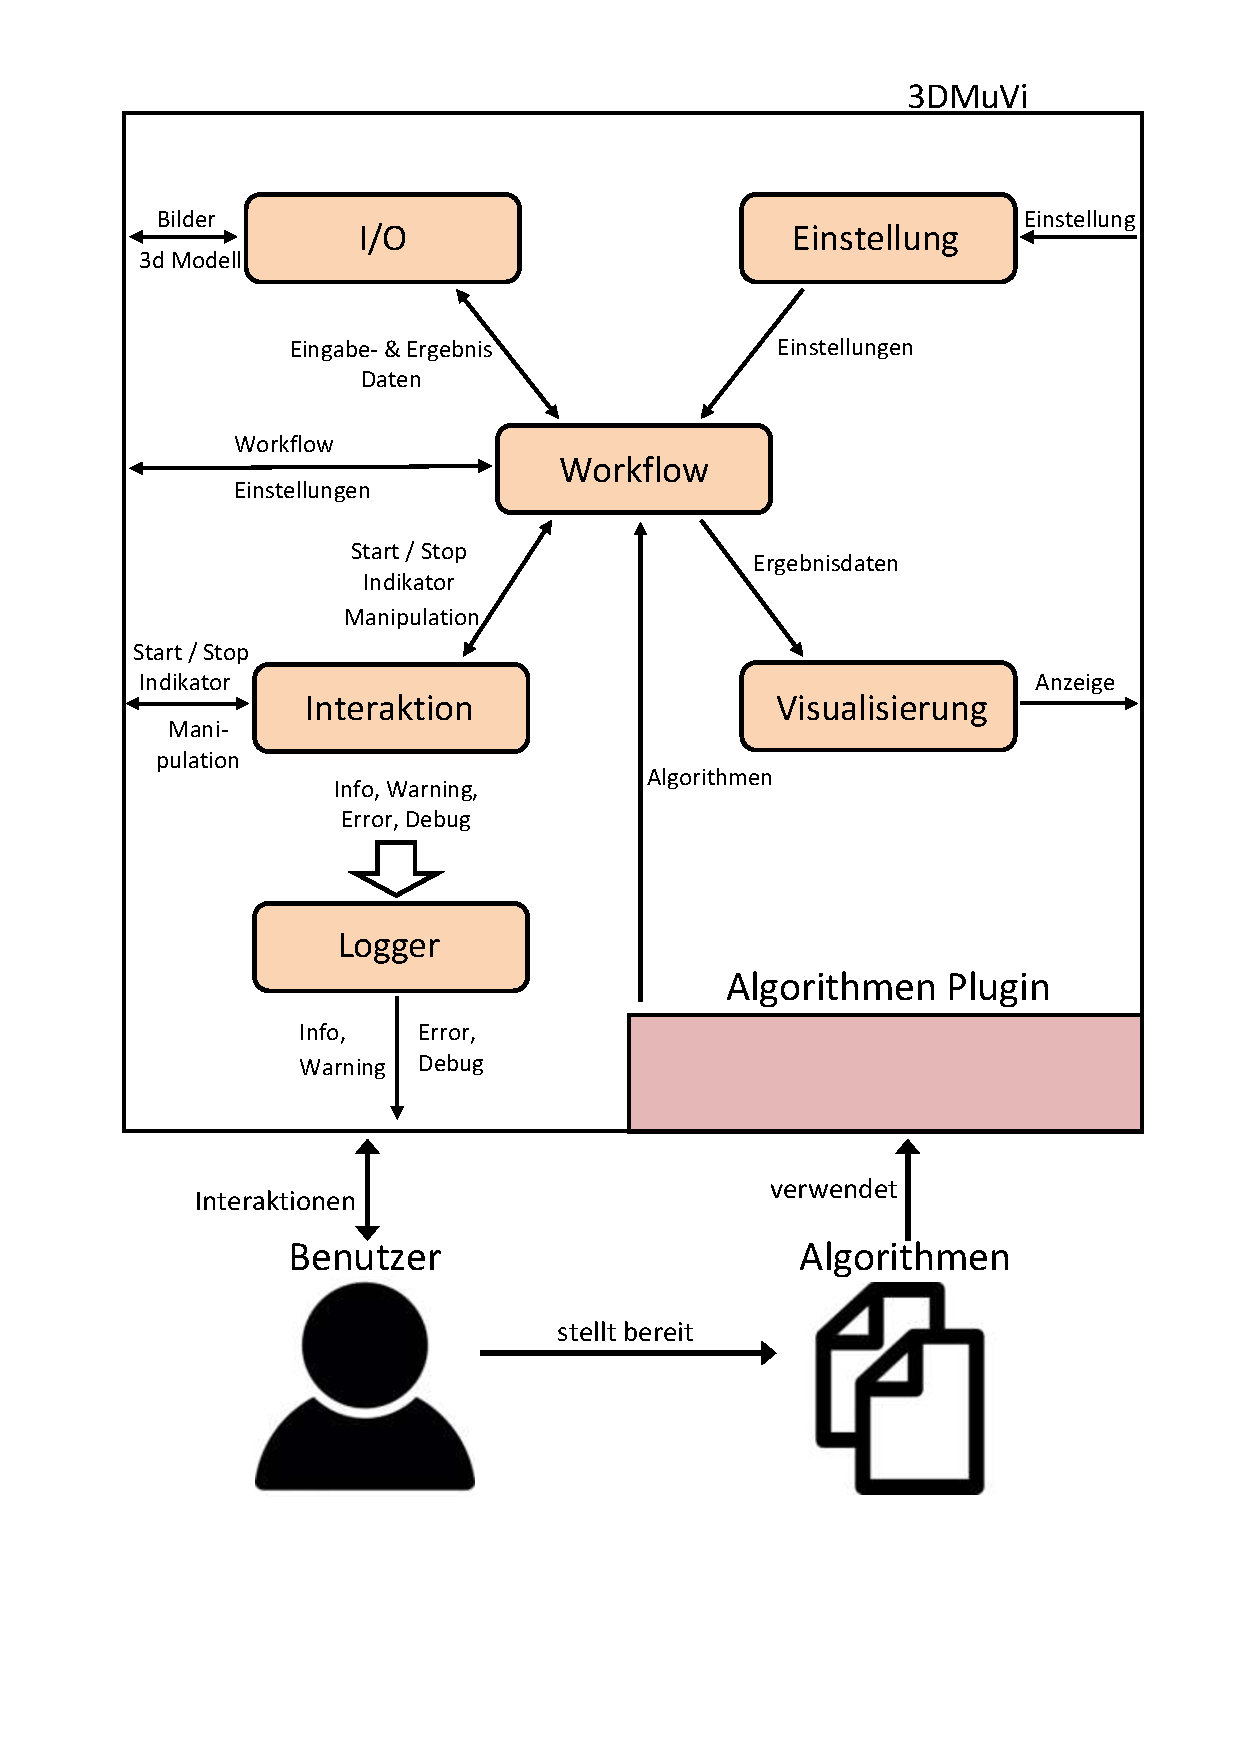
\includegraphics[width=0.87\textwidth]{img/Datenflussuebersicht.pdf}
\newpage
\section{Architektur}
Die Architektur orientiert sich am Systemodell. 5 der 6 Module bleiben bestehen und werden in Pakete weiter aufgeteilt. Als Hauptentwurfsmuster wird MVC verwendet.
Aufgrund der starken Abhängigkeit von Interaktion und Visualisierung wird dies in das gemeinsame Modul GUI fusioniert. 
\subsection{GUI}
Die GUI besteht aus dem Modul Interaktion und dem Modul Visualisierung.
Sie stellt eine voll Funktionsfähige GUI da, welche die Daten Visualisiert und auf Benutzereingaben reagiert.
\subsection{Workflow}
Der Workflow interagiert mit den Algorithmen Plugins und führt diese aus.
\subsection{Logger}
Der Logger speichert die Logdaten der Algorithmen und liefert sie an die GUI
\subsection{Einstellungen}
Die Einstellungen verwalten die Globalen Einstellungen und die Parameter der Algorithmen.
\subsection{I/O}
Die I/O stellt Methoden zum ein und auslesen bereit.
